\section{Tulokset}

Kuvissa \ref{fig:mfix} ja \ref{fig:mfree} on simuloitu MUSIC-algoritmia sekä kiinnitetyllä että vapaalla orientaatiolla. Simuloinneissa kolme lähdedipolia sijoitettiin aivokuorelle, jotka on merkitty punaisina ympyröinä ja topografia on muodostettu MUSIC-algoritmin paikannusfunktion arvoista.

Kuvissa \ref{fig:RAPfix} ja \ref{fig:RAPfree} on simuloitu RAP-MUSIC- algoritmia kiinnitetyllä ja vapaalla orientaatiolla. Kuvissa musta rasti kuvaa paikannusfunktion maksimiarvon paikkaa ja löydetyt dipolit merkataan punaisella neliöllä.

Kuvista huomataan, että MUSIC vapaalla orientaatiolla saa aikaan suurempia aktiivisuuden alueita kuin kiinnitetyllä orientaatiolla, mikä vaikeuttaa lähteiden tarkkaa paikantamista. 

Tavallisen MUSIC-algoritmin yksi ongelmista on oikeiden lähteiden erottaminen vääristä \citep{Mosher1998RecursiveLocalization}. Lisäksi MUSIC-algoritmilla on vaikeuksia löytää synkronoituja lähteitä \citep{Mosher1999SourceMUSIC}. RAP- sekä TRAP-MUSIC-algoritmeilla vaikeuksia löytää hyvin lähellä toisiaan olevia dipoleita. Löydettyä lähdettä projisoidessa pois häviää myös löytämättä jääneen lähteen komponentteja.

\clearpage
\begin{figure}[h]
    \centering
    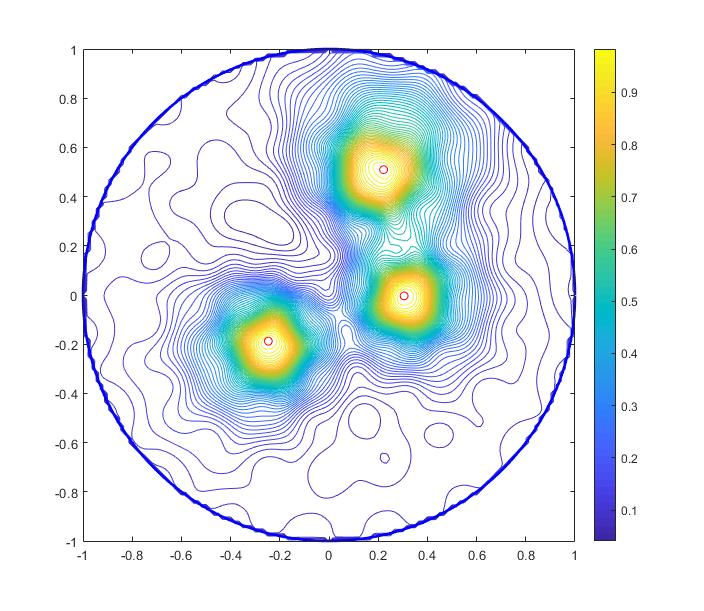
\includegraphics[scale=0.38]{mfix.jpg}
    \caption{MUSIC-algoritmin simulointi pallomallilla kiinnitetyllä orientaatiolla.}
    \label{fig:mfix}
\end{figure}

\begin{figure}[h]
    \centering
    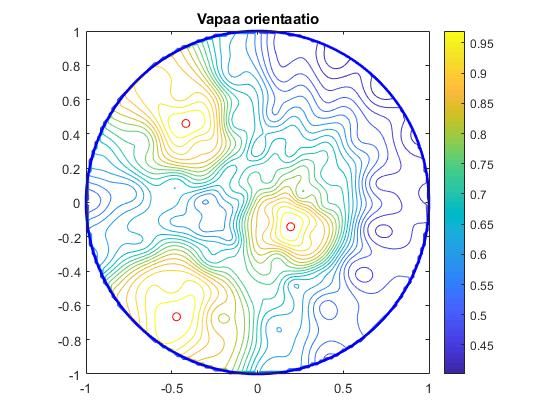
\includegraphics[scale=0.41]{mfree.jpg}
    \caption{MUSIC-algoritmin simulointi pallomallilla vapaalla orientaatiolla.}
    \label{fig:mfree}
\end{figure}

\clearpage

\begin{figure}[ht]
    \centering
    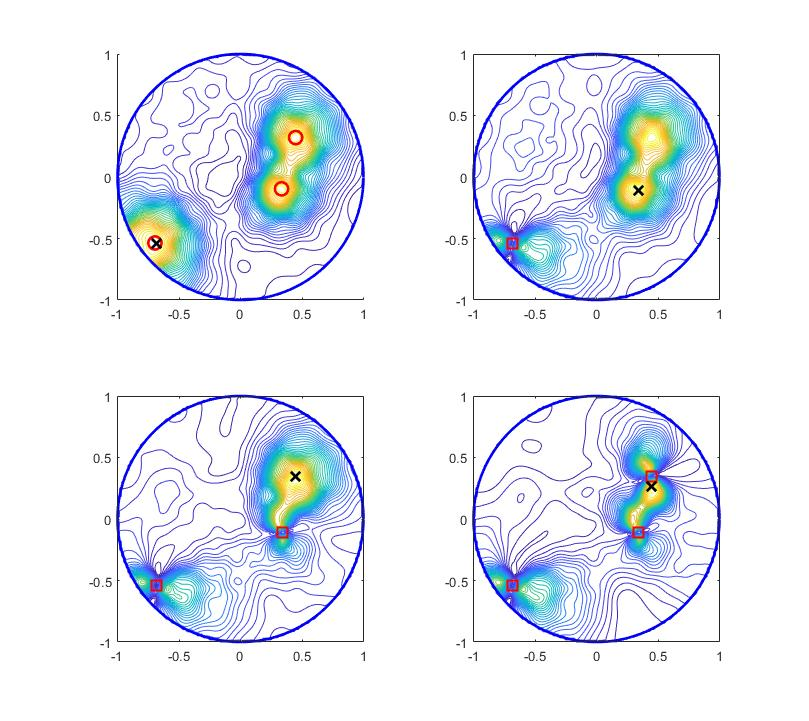
\includegraphics[width=\textwidth]{RAPfixed.jpg}
    \caption{RAP-MUSIC kiinnitetyllä orientaatiolla}
    \label{fig:RAPfix}
\end{figure}

\clearpage
\begin{figure}[ht]
    \centering
    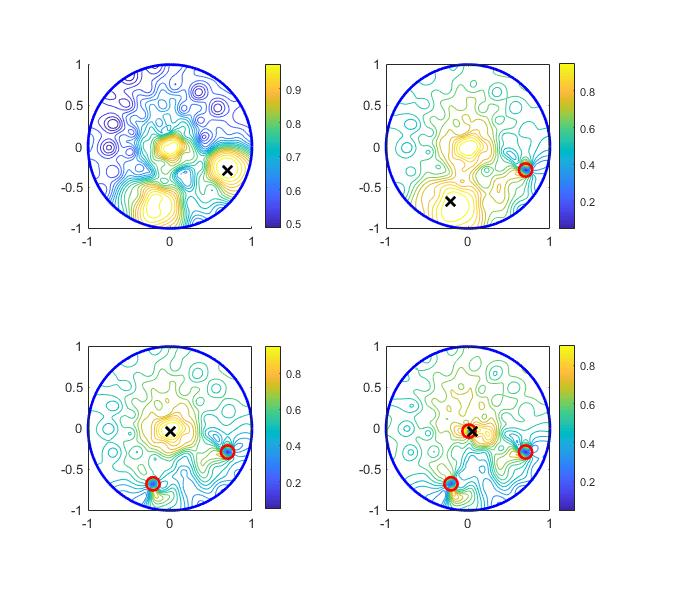
\includegraphics[width=\textwidth]{RAPfree.jpg}
    \caption{RAP-MUSIC vapaalla orientaatiolla}
    \label{fig:RAPfree}
\end{figure}